\emph{On note $E$ l'évènement \og le patient est un enfant \fg{} et $M$ l'évènement \og le médecin prescrit des
médicaments \fg. On a $P(E) = 0,7$, $P_E(M) = 0,2$ et $P_{\overline{E}}(M) = 0,4$.}

\begin{enumerate}
	\item La somme des probabilités issues d'un
	même n{\oe}ud vaut 1 : $P(\overline{E}) = 1 - 0,7 = 0,3$,
	$P_E(\overline{M}) = 1 - 0,2 = 0,8$ et $P_{\overline{E}}(\overline{M}) = 1 - 0,4 = 0,6$.

	\begin{center}
		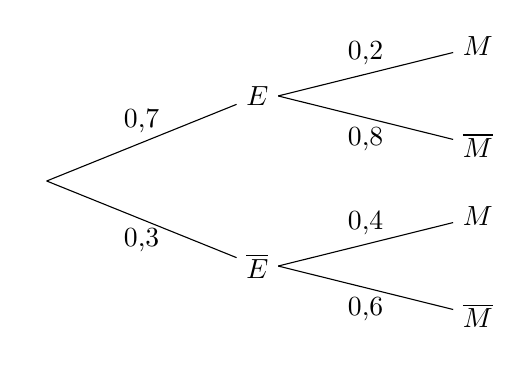
\begin{tikzpicture}[x=2.8cm, y=0.9cm]
			
			\node (root) at (0,0) {};
			\node (E) at (1,1.2) {$E$};
			\node (Eb) at (1,-1.2) {$\overline{E}$};
			\node (M1) at (2,1.9) {$M$};
			\node (M1b) at (2,0.5) {$\overline{M}$};
			\node (M2) at (2,-0.5) {$M$};
			\node (M2b) at (2,-1.9) {$\overline{M}$};
			
			\draw (root.east) -- (E) node[pos=0.5,above] {0,7};
			\draw (root.east) -- (Eb) node[pos=0.5,below] {0,3};
			
			\draw (E.east) -- (M1) node[pos=0.5,above] {0,2};
			\draw (E.east) -- (M1b) node[pos=0.5,below] {0,8};
			\draw (Eb.east) -- (M2) node[pos=0.5,above] {0,4};
			\draw (Eb.east) -- (M2b) node[pos=0.5,below] {0,6};
		\end{tikzpicture}
	\end{center}

	\item La probabilité d'un chemin de l'arbre est le produit des probabilités rencontrées le
	long de ce chemin :
	\[P(\overline{E} \cap M) = P(\overline{E}) \times P_{\overline{E}}(M) = 0,3 \times 0,4 = 0,12.\]
	La probabilité que le patient choisi soit un \textbf{adulte} \textbf{et} que le médecin lui prescrive des médicaments est de $0,12$ ;
	autrement dit, 12\,\% des patients sont des adultes à qui le médecin prescrit des médicaments.
	

	\item $E$ et $\overline{E}$ forment une partition de l'univers. D'après la formule des
	probabilités totales :                          
	
	 \[ P(M) = P(E \cap M) + P(\overline{E} \cap M) \]
 \[ P(M) = P(E) \times P_E(M) + P(\overline{E} \cap M) \]
 \[ P(M) = 0,7 \times 0,2 + 0,12 \]
 \[P(M) =  0,26\]
	
	La probabilité que le médecin prescrive des médicaments au patient est égale à $0,26$.
	

	\item Deux évènements $E$ et $M$ (avec $P(E) \neq 0$) sont indépendants si et seulement si
	
	$P(E \cap M) = P(E) \times P(M)$.

	D'une part $P(E \cap M) = 0,14$ ; d'autre part
	$P(E) \times P(M) = 0,7 \times 0,26 = 0,182$.

	Comme $0,14 \neq 0,182$, l'égalité n'est pas vérifiée. 

	Les évènements $E$ et $M$ ne sont \textbf{pas indépendants}.


	\item On cherche la probabilité conditionnelle $P_M(E)$.
	\[P_M(E) = \dfrac{P(E \cap M)}{P(M)} = \dfrac{0,14}{0,26} = \dfrac{14}{26} = \dfrac{7}{13}.\]
	Sachant que le médecin a prescrit des médicaments, la probabilité que le patient soit un
	enfant est égale à $\dfrac{7}{13}$.
\end{enumerate}
